\documentclass[UTF8,a4paper,11pt,fontset=windows]{ctexart}
\usepackage[margin=2.3cm]{geometry}
\usepackage{amsmath,amssymb,booktabs,array,graphicx,subcaption,float,hyperref,xcolor}
\hypersetup{colorlinks=true,linkcolor=black,urlcolor=blue!55!black}
\setlength{\parindent}{2em}
\setlength{\parskip}{0.25em}
\renewcommand{\arraystretch}{1.2}
\newcommand{\pct}{\%}
\newcommand{\MainEpisodes}{90}
\newcommand{\MainCorrectCount}{87}
\newcommand{\MainFailureCount}{3}
\newcommand{\MainRecognitionPct}{100.0}
\newcommand{\MainGraspPct}{100.0}
\newcommand{\MainSortPct}{96.7}
\newcommand{\MainPositionMm}{2.75}
\newcommand{\MainCycleSec}{10.85}
\newcommand{\MainMeanOmega}{7.00}
\newcommand{\MainMaxOmega}{51.55}
\newcommand{\MainMeanRelative}{28.57}
\newcommand{\MainMaxRelative}{179.68}
\newcommand{\MainCubeCorrect}{30}
\newcommand{\MainCylinderCorrect}{30}
\newcommand{\MainPrismCorrect}{27}
\newcommand{\TruthCorrectCount}{79}
\newcommand{\TruthSortPct}{87.8}
\newcommand{\TruthCycleSec}{10.83}
\newcommand{\TruthPrismCorrect}{19}
\newcommand{\SpeedSlowCorrectCount}{28}
\newcommand{\SpeedSlowSortPct}{93.3}
\newcommand{\SpeedSlowPositionMm}{2.49}
\newcommand{\SpeedSlowCycleSec}{11.52}
\newcommand{\SpeedFastCorrectCount}{29}
\newcommand{\SpeedFastSortPct}{96.7}
\newcommand{\SpeedFastPositionMm}{2.42}
\newcommand{\SpeedFastCycleSec}{10.51}
\newcommand{\LightDimCorrectCount}{28}
\newcommand{\LightDimSortPct}{93.3}
\newcommand{\LightDimPositionMm}{2.39}
\newcommand{\LightDimCycleSec}{10.83}
\newcommand{\DemoCubeOmega}{0.74}
\newcommand{\DemoCylinderOmega}{0.70}
\newcommand{\DemoPrismOmega}{0.69}


\title{\vspace{2.6cm}\Huge 基于机器视觉的间歇式物料传输线零件识别与抓取系统设计\\[0.8cm]
\Large 《机器视觉及其应用》课程项目设计报告}
\author{项目组}
\date{2026年9月23日}

\begin{document}
\pagestyle{plain}
\maketitle
\fontsize{12pt}{17.5pt}\selectfont
\thispagestyle{empty}
\vfill
\clearpage
\begingroup
\fontsize{13pt}{19pt}\selectfont
\tableofcontents
\endgroup
\clearpage

\section{概述}
针对输送线中不同零件的自动分拣需求，我们设计了一套基于固定 RGB 相机与双指夹爪的间歇式识别抓取系统。该系统中，红色立方体、绿色圆柱体和蓝色三棱柱依次进入识别区域；输送带停止后，系统利用 OpenCV 提取零件轮廓并估计其平面中心，再由 Franka Panda 机械臂完成抓取和分类投放。我们采取间歇运行，这使图像采集与机械臂作业发生在相对静止的工况下，便于分析定位误差与抓取结果之间的关系。

系统在 MuJoCo 中构建输送带、固定相机、标定点、零件及料箱场景，以 Menagerie 提供的 Panda 机械臂及原生双指夹爪为执行机构\cite{menagerie,panda}。视觉处理采用颜色分割、轮廓分析和四点单应性标定；运动控制采用阻尼最小二乘逆运动学、关节闭环到位和有限状态机。抓取流程中，使用 RGB 图像估计的类别与位置，并使用仿真中获取的真值进行误差统计及单独设置的位置对照实验。最后，我们通过随机初始化实验评价识别、定位、抓取、分类及周期等性能，并分析三棱柱抓取中的转动与投放误差。

\section{系统的作业流程与评价指标}
一轮作业从上料开始，依次完成动作如下：输送、停带、识别、预抓取、下降、双指闭合、抬升、转运、下降投放、张爪、撤离和核验，而系统则会在每轮记录如下内容：真实类别与识别类别、平面定位误差、抬升结果、投放位置、失败类型及周期。当零件中心在抬升后达到 $0.24$ m 高度时，系统判定该轮抓取成功；当类别判断正确，且零件最终中心位于对应料箱中心 $\pm0.065$ m 的平面范围内、高度低于 $0.13$ m 时，判定为正确分类投放。对于各项成功率的计算，我们采用该组实验的全部回合数作为分母。

表\ref{tab:goals}列出系统的设计指标与双指夹爪主实验结果。结果显示，识别、定位、抬升与分类投放达到设定指标，平均周期则略微超过 $8$ s；这里将在后文结合控制流程分析周期较长的原因。
\enlargethispage{1.5\baselineskip}

\begin{table}[H]\centering\small
\caption{设计目标与\MainEpisodes 次视觉控制主实验结果}\label{tab:goals}
\begin{tabular}{lcc}
\toprule 指标 & 设计目标 & 实测值\\\midrule
三类识别准确率 & $\geq95\pct$ & \MainRecognitionPct\pct\\
平面定位平均欧氏误差 & $\leq5$ mm & \MainPositionMm\ mm\\
抬升成功率 & $\geq90\pct$ & \MainGraspPct\pct\\
正确分类投放率 & $\geq90\pct$ & \MainCorrectCount/\MainEpisodes，\MainSortPct\pct\\
平均单次周期 & $\leq8$ s & \MainCycleSec\ s\\
随机初始化主实验 & $\geq90$ 次 & \MainEpisodes\ 次\\\bottomrule
\end{tabular}
\end{table}

\section{系统架构、器件选型与参数计算}
\subsection{系统架构}
我们在 MuJoCo 3.11 中搭建仿真场景如下：输送带利用环境中静态几何体的 \texttt{surfacevel} 属性实现表面运动，再用物理引擎计算零件与输送带、夹爪之间的接触\cite{mujoco_xml}。我们固定俯视 RGB 相机以 $640\times480$ 的分辨率采集图像，而执行机构则为七自由度 Panda 机械臂及其对应的原生双指夹爪，对于该夹爪，控制信号范围为 $0\sim255$，其中 $255$ 对应张开、$0$ 对应闭合，对应单侧手指行程为 $0\sim0.04$ m。

我们将抓取中心 \texttt{grasp\_center} 设在 Panda \texttt{hand} 局部坐标系的 $z=0.103$ m 处，使其高度与原模型指尖碰撞垫片中心的约 $0.1029$ m 相对应。对于指尖夹持接触的阻滑能力的表征，分别取滑动摩擦 $2.5$、扭转摩擦 $0.02$ 和滚动摩擦 $0.001$。图\ref{fig:scene}展示系统场景。

\begin{figure}[H]\centering
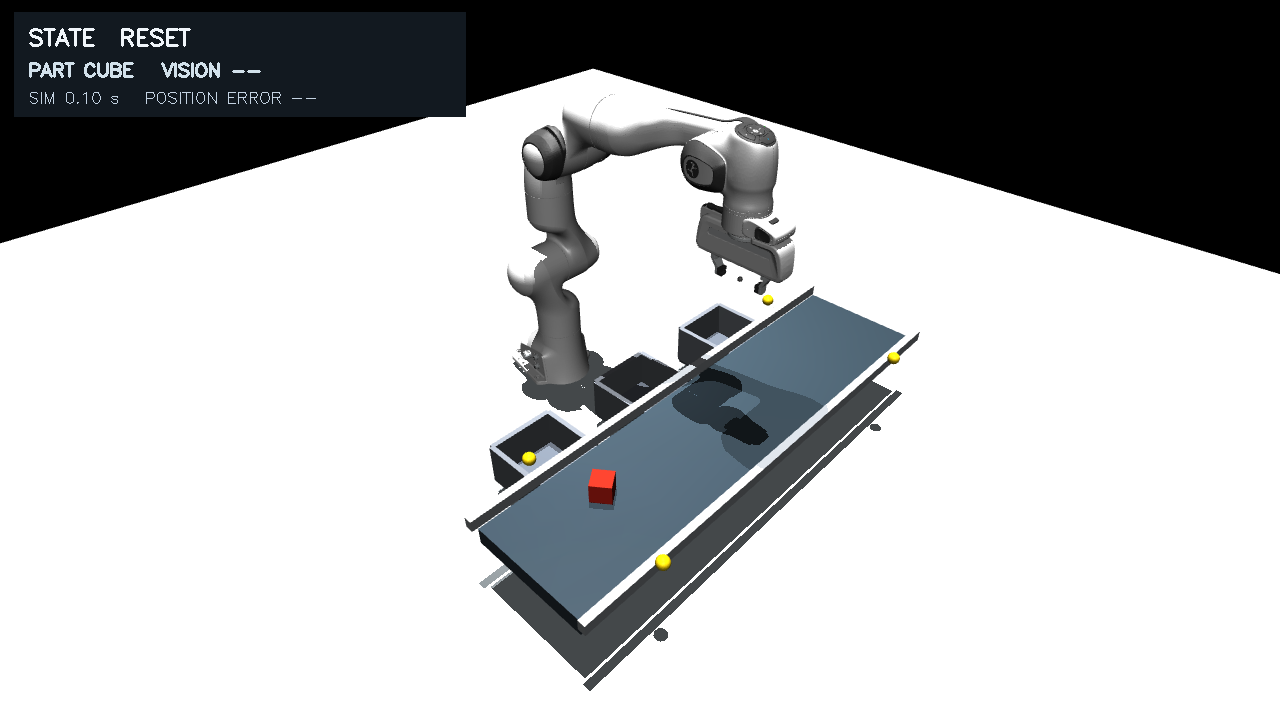
\includegraphics[width=0.91\linewidth]{../outputs/gripper_demo_cube/scene.png}
\caption{系统仿真场景：Panda 机械臂、间歇式输送带、四个标定点、料箱与待输送零件}\label{fig:scene}
\end{figure}

\subsection{几何参数、负载与相机}
输送带的带体中心位于 $(0.55,0,0.14)$ m，半宽为 $0.14$ m、半长为 $0.56$ m，带面约位于 $z=0.16$ m。立方体边长为 $46$ mm；圆柱体直径为 $44$ mm、高 $46$ mm；三棱柱平面三角截面横向约 $48$ mm、厚 $36$ mm。三类零件的质量均设为 $35$ g，其重力约为
\begin{equation}
G=mg=0.035\times9.81\approx0.343\ {\rm N}.
\end{equation}
按两侧对称夹持、库仑摩擦平衡重力的准静态条件估算，单侧法向力需满足 $N\geq G/(2\mu)$。将模型滑动摩擦系数 $\mu=2.5$ 代入后，得到理想条件下的静态下限 $N\geq0.069$ N。

顶部相机位于 $(0.50,-0.04,1.26)$ m，竖直视场角为 $55^\circ$。以带面为近似平面时，相机与带面的高度差为 $h=1.10$ m，由此估计的竖直覆盖范围为
\begin{equation}
H=2h\tan(55^\circ/2)\approx1.145\ {\rm m},\qquad H/480\approx2.39\ {\rm mm/pixel}.
\end{equation}
四个黄色标记的平面坐标为 $(0.37,\pm0.40)$ m、$(0.73,\pm0.40)$ m；\newline 三个料箱的中心分别位于 $(0.30,-0.31)$、$(0.30,0)$、$(0.30,0.31)$ m。

\subsection{带速与动作参数}
在主实验中，我们将输送带速度设为 $v=0.12$ m/s，带面运动约 $1.35$ s，对应位移 $s=vt=0.162$ m。带面速度归零后，系统等待 $0.25$ s 再采集识别图像，仿真步长为 $0.004$ s。

本场景采用瞬时停带模型；实体输送机构的制动位移可按 $s_{\rm stop}=v^2/(2a)$ 估算。预抓取和转运阶段的抓取中心目标高度约为 $0.34$ m；下降夹持时，立方体与圆柱体的目标高度为 $0.185$ m，三棱柱为 $0.180$ m，投放高度为 $0.17$ m。普通运动的关节命令限速为 $0.8$ rad/s，带物转运时降至 $0.35$ rad/s。

\section{算法与控制}
\subsection{形色识别与四点标定}
系统中，我们先用视觉算法将相机采集的 RGB 图像转换至 HSV 空间，分别生成红、绿、蓝三类颜色掩膜。随后，算法对掩膜进行形态学处理和轮廓面积筛选，利用轮廓圆度与多边形近似顶点数辅助判断零件形状，并通过图像矩求取目标中心像素 $(u,v)$。我们根据四个黄色标定点的图像位置与已知平面坐标计算单应性矩阵 $H$，使图像点与带面位置满足
\begin{equation}
\lambda[x,y,1]^{\mathsf T}=H[u,v,1]^{\mathsf T}.
\end{equation}
单应性变换采用 OpenCV 的平面映射形式\cite{opencv_h}。图\ref{fig:detection}中，选取三棱柱展示其识别的轮廓、中心及类别的识别结果。这之后，系统将识别类别与标定后的平面坐标一并传给机械臂控制流程，用于确定抓取目标。

\begin{figure}[H]\centering
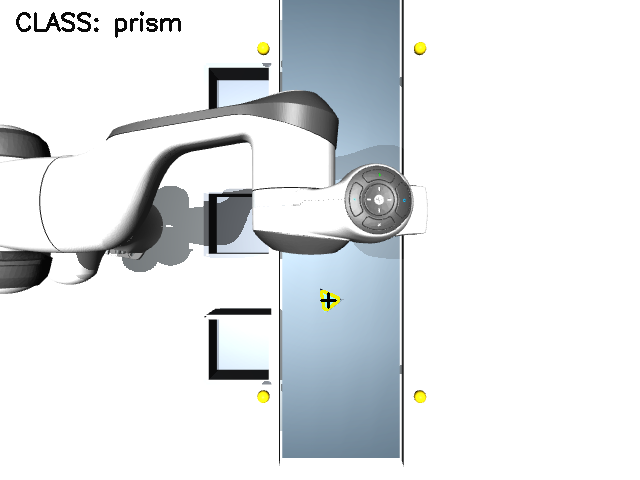
\includegraphics[width=0.65\linewidth]{../outputs/gripper_demo_prism/detection.png}
\caption{三棱柱 RGB 图像的轮廓、中心与类别识别结果}\label{fig:detection}
\end{figure}

\subsection{逆运动学}
机械臂保持末端向下的初始姿态，并以 \texttt{grasp\_center} 为末端目标。对于七个关节构成的 $6\times7$ 雅可比矩阵 $J$，控制器采用阻尼最小二乘法更新关节角：
\begin{equation}
\Delta q=J^{\mathsf T}(JJ^{\mathsf T}+\lambda^2I)^{-1}e,\qquad \lambda=0.035.
\end{equation}
对于每次关节动作，逆运动学迭代将关节增量限制在 $\pm0.075$ rad 内，并遵守模型的关节限位。执行运动时，控制器对关节命令施加速度约束；当机械臂接近目标后，再根据末端实测雅可比和位置偏差进行局部修正，以减小关节动态误差造成的抓取偏移。当平面位置误差小于 $3$ mm、垂向误差小于 $8$ mm，且关节命令与实际关节角之差小于 $0.02$ rad 时，状态机将会切换至下一阶段；如果机械臂运动到位但超时，则自动进入张爪与撤离流程。

\subsection{双指夹持状态机}
双指夹持的状态机如下：
\begin{center}\small\ttfamily
RESET -- CONVEY -- DETECT -- PREGRASP -- DESCEND\\
CLOSE -- LIFT -- TRANSFER -- LOWER -- OPEN\\
RETRACT -- VERIFY -- RETURN
\end{center}

在下降阶段，夹爪保持张开。双指闭合后，系统先检查接触数据；确认左右两指均与零件接触后，机械臂才开始抬升。带物转运时，关节限速降至 $0.35$ rad/s，以减小加速度引起的滑移。

对于本系统，目标失检、逆运动学求解失败、到位超时或单侧接触，都会触发 \texttt{SAFE\_OPEN} 和 \texttt{SAFE\_RETRACT} 安全流程。本实验根据抬升高度和最终入箱位置评价抓取与投放结果，分类错误的回合计入错误投放。

\begin{figure}[H]\centering
\begin{subfigure}{0.42\linewidth}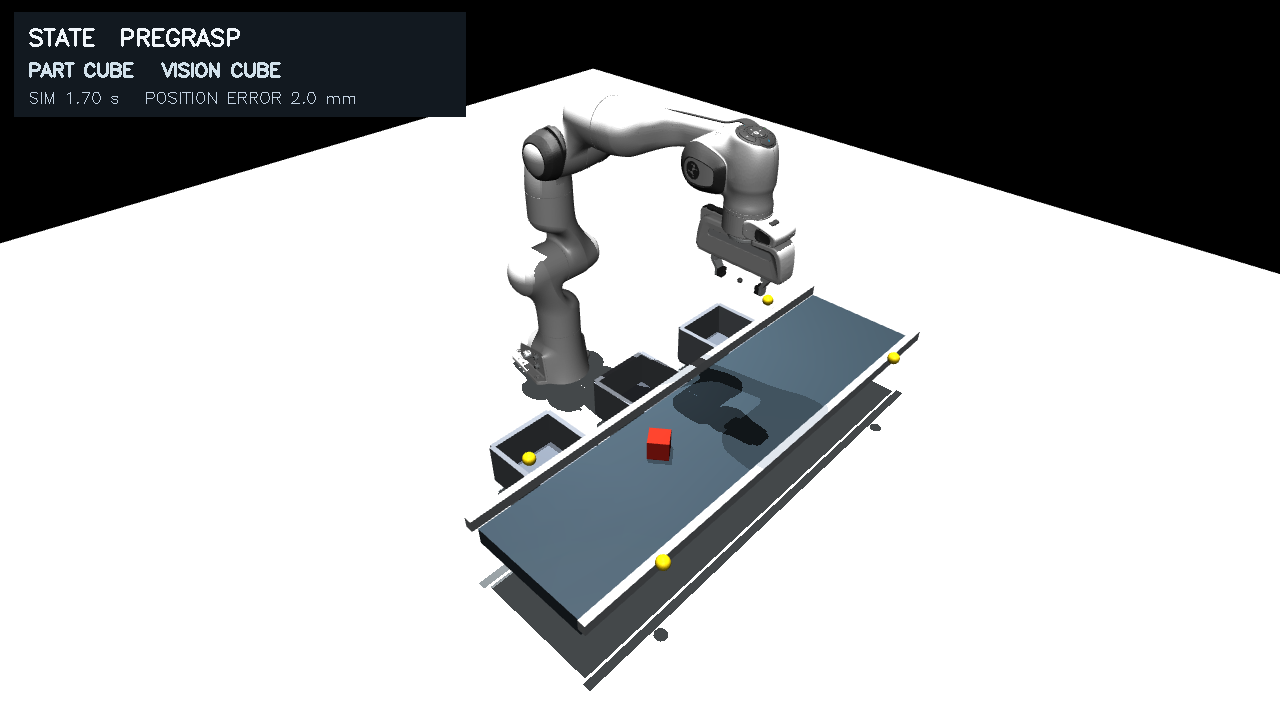
\includegraphics[width=\linewidth]{../outputs/gripper_demo_cube/pregrasp.png}\caption{预抓取入口}\end{subfigure}\hfill
\begin{subfigure}{0.42\linewidth}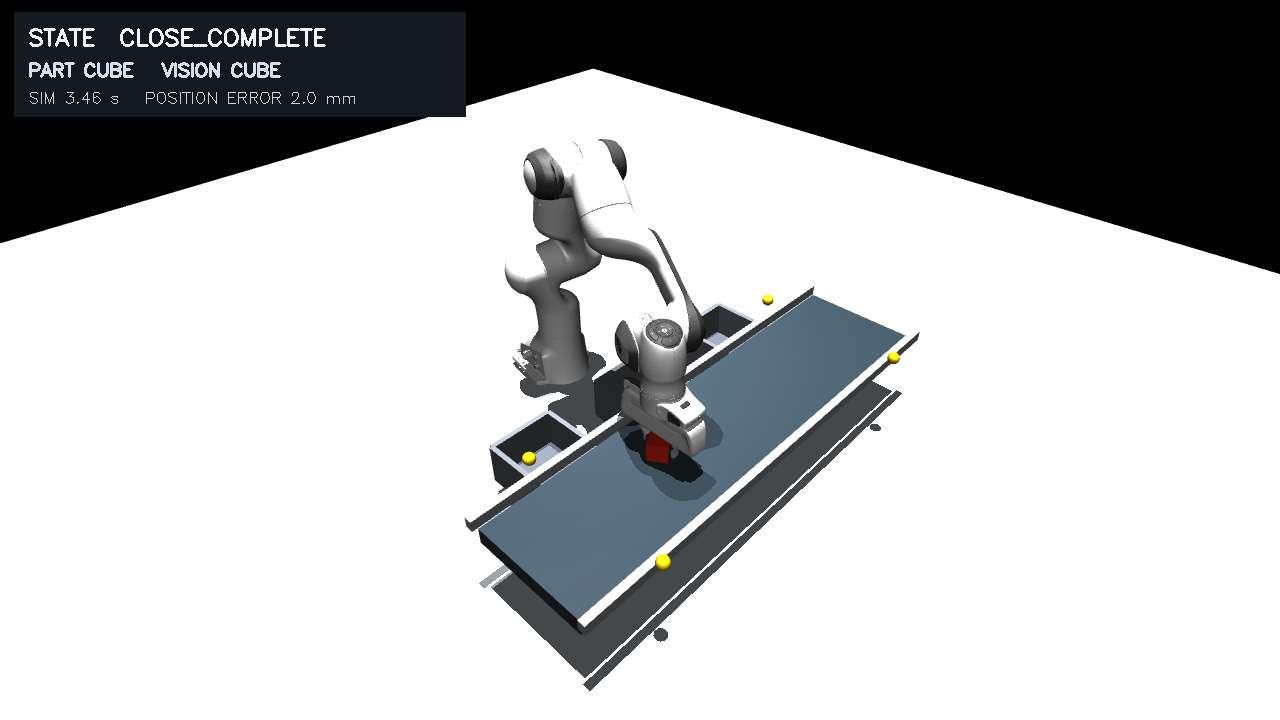
\includegraphics[width=\linewidth]{../outputs/gripper_demo_cube/close.png}\caption{双指闭合完成}\end{subfigure}\\[0.18cm]
\begin{subfigure}{0.42\linewidth}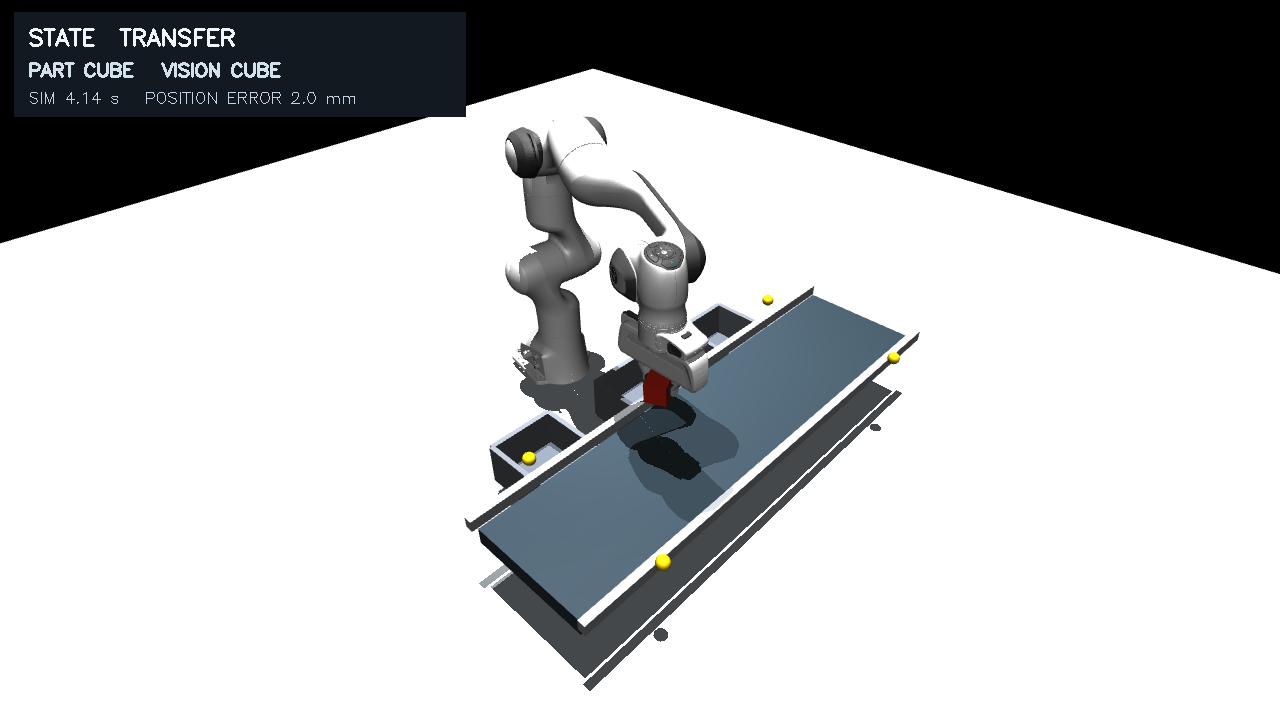
\includegraphics[width=\linewidth]{../outputs/gripper_demo_cube/transfer.png}\caption{转运入口}\end{subfigure}\hfill
\begin{subfigure}{0.42\linewidth}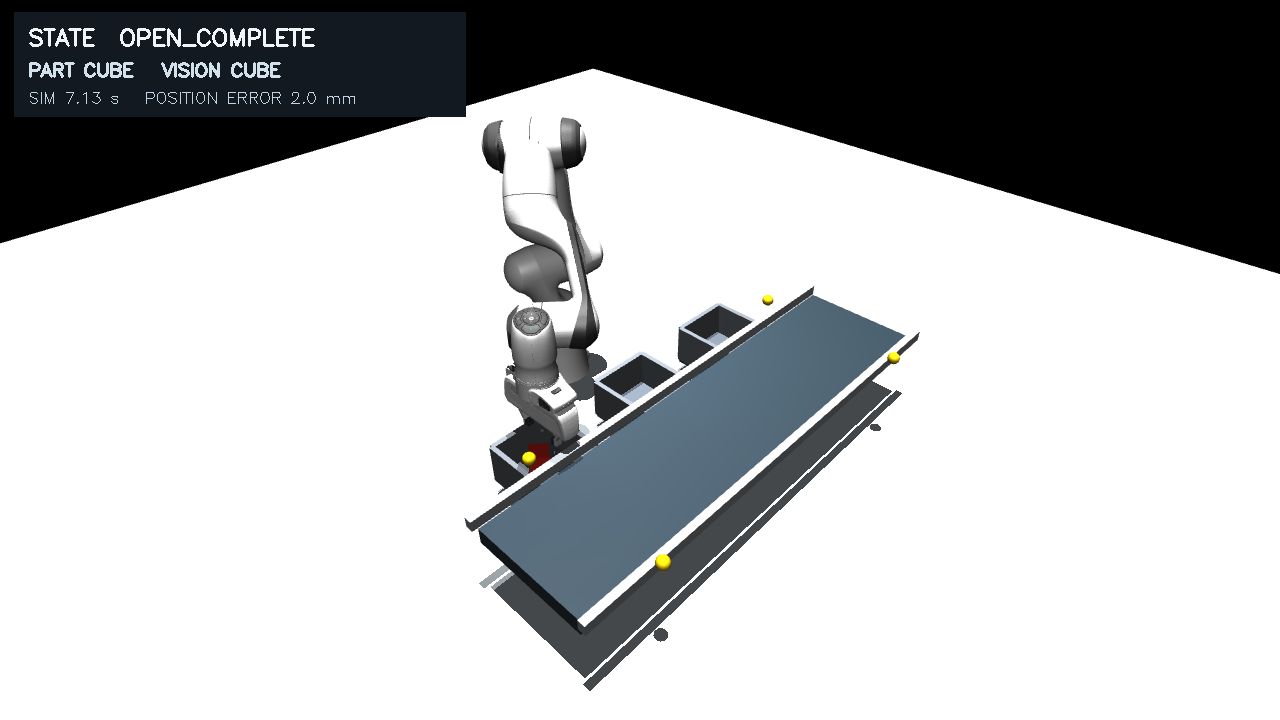
\includegraphics[width=\linewidth]{../outputs/gripper_demo_cube/open.png}\caption{料箱上方张爪完成}\end{subfigure}
\caption{同一抓取回合的关键阶段}\label{fig:stages}
\end{figure}

图\ref{fig:stages}展示同一回合的预抓取、闭合、转运及投放阶段。夹爪闭合时，零件位于双指之间。转运结束后，机械臂在目标料箱上方张爪释放零件。
\enlargethispage{2\baselineskip}

\section{实验设计、结果与分析}\label{sec:experiment}
\subsection{实验设置与统计}
主实验使用了90个连续种子，共进行 \MainEpisodes\ 个随机初始化回合，三类零件各 $30$ 个。每轮实验随机改变零件的横向位置、纵向偏差和平面朝向。

为了分析位置估计对分拣结果的影响，我们用相同种子另设 $90$ 个真值位置对照回合，带速 $0.08$、$0.16$ m/s 和光照比例 $0.6$ 的条件实验各进行 $30$ 次。所有实验均依据 RGB 图像识别和定位，真值位置组仅用仿真平面位置替换视觉定位结果。

我们的实验采用以下指标评价系统性能：类别识别准确率、平面定位误差、抬升成功率、正确入箱率和单轮周期。为了分析夹持稳定性，系统还在 \texttt{LIFT} 与 \texttt{TRANSFER} 阶段采样零件角速度和相对手部姿态，将相对姿态定义为 $R_{\rm rel}=R_{\rm hand}^{\mathsf T}R_{\rm part}$。

\subsection{视觉主实验}
在 \MainEpisodes\ 次视觉主实验中，系统正确识别零件类别 \MainEpisodes/\MainEpisodes，成功抬升 \MainEpisodes/\MainEpisodes，正确分类投放 \MainCorrectCount/\MainEpisodes。平面定位平均误差为 \MainPositionMm\ mm，平均周期为 \MainCycleSec\ s。

按零件类别统计，立方体、圆柱体和三棱柱的正确投放结果分别为 \MainCubeCorrect/30、\MainCylinderCorrect/30 和 \MainPrismCorrect/30。全部 \MainFailureCount\ 次错误均发生在三棱柱投放判定中。图\ref{fig:charts}展示了识别、定位、成功率与周期分布，图\ref{fig:failure}则展示其中一个失败回合的最终状态：系统完成识别和抬升后，三棱柱落在目标料箱的判定范围外。

\begin{figure}[H]\centering
\begin{subfigure}{0.40\linewidth}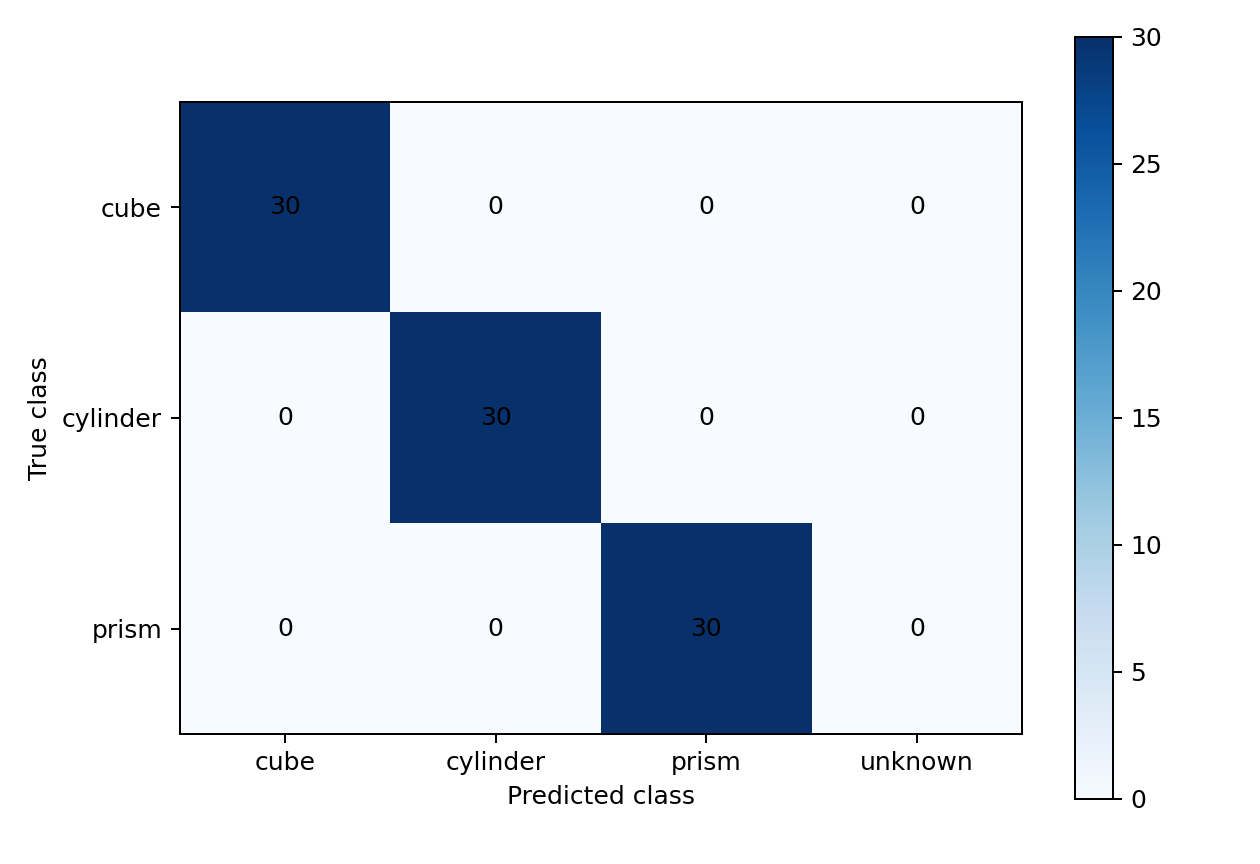
\includegraphics[width=\linewidth]{../outputs/gripper_main/confusion.png}\caption{类别混淆矩阵}\end{subfigure}\hfill
\begin{subfigure}{0.40\linewidth}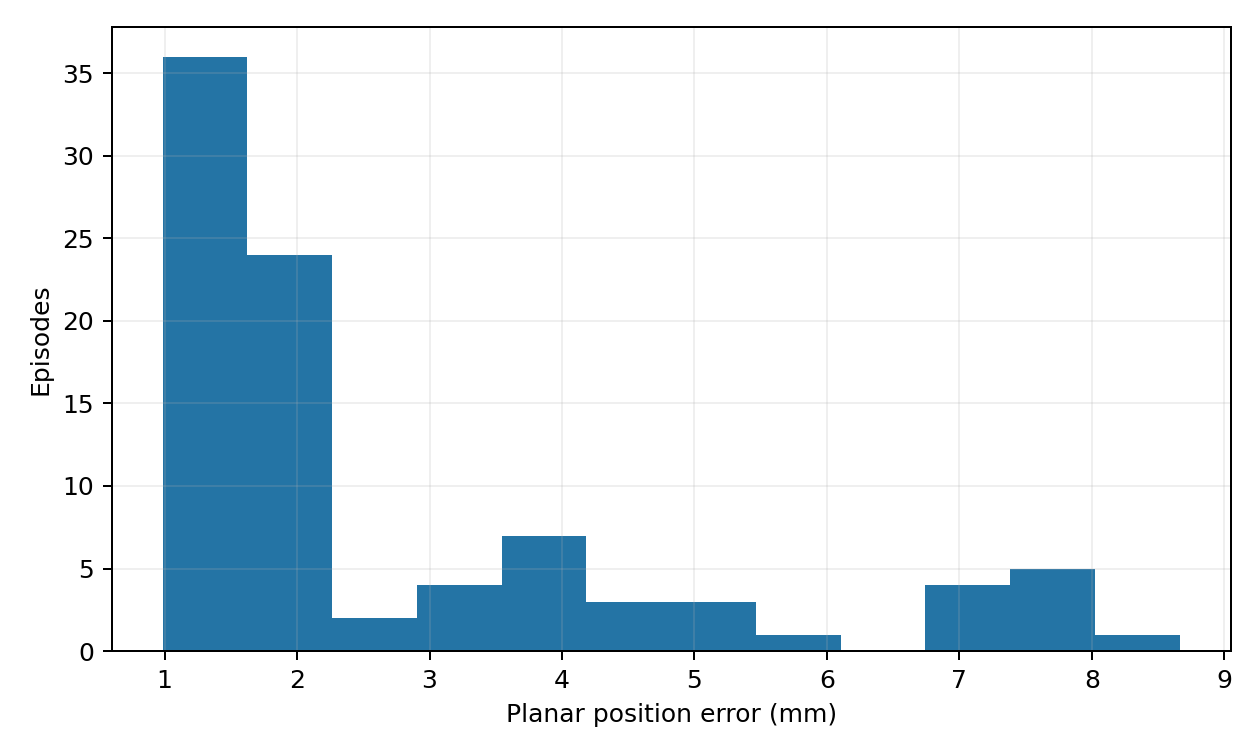
\includegraphics[width=\linewidth]{../outputs/gripper_main/position_error.png}\caption{平面定位误差}\end{subfigure}\\[0.15cm]
\begin{subfigure}{0.40\linewidth}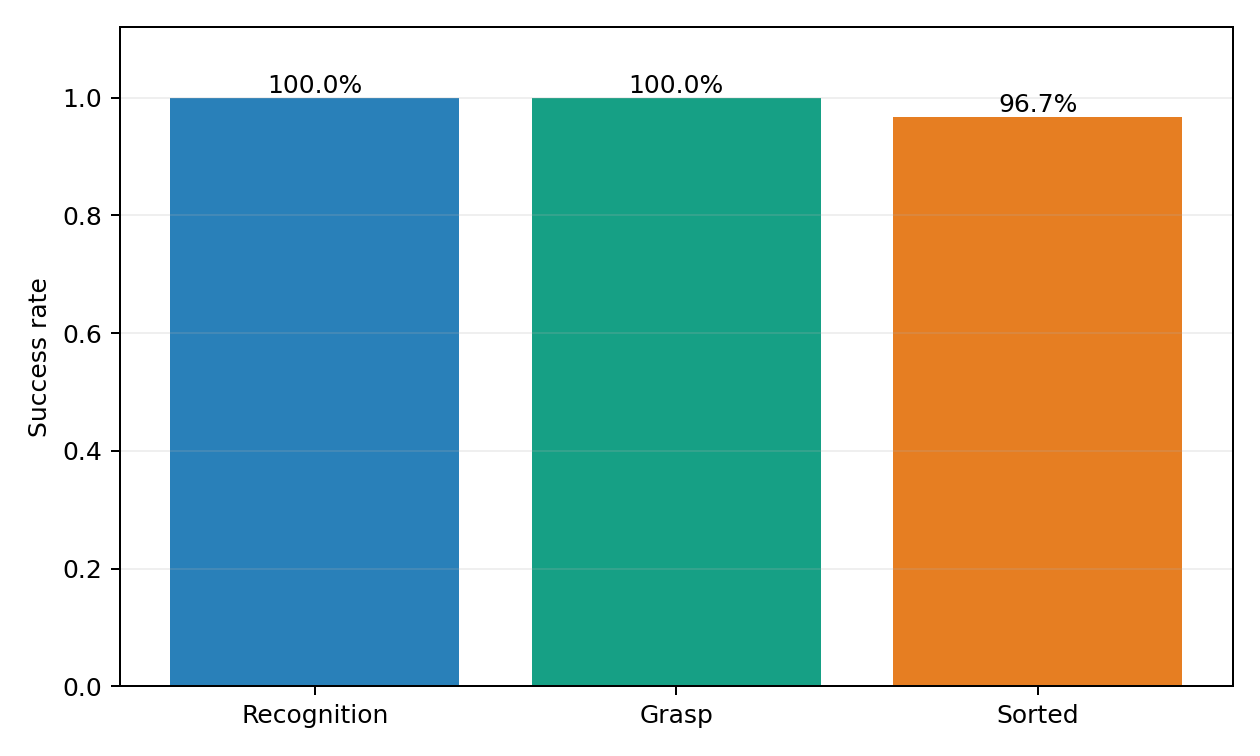
\includegraphics[width=\linewidth]{../outputs/gripper_main/success_rates.png}\caption{识别、抬升与正确入箱}\end{subfigure}\hfill
\begin{subfigure}{0.40\linewidth}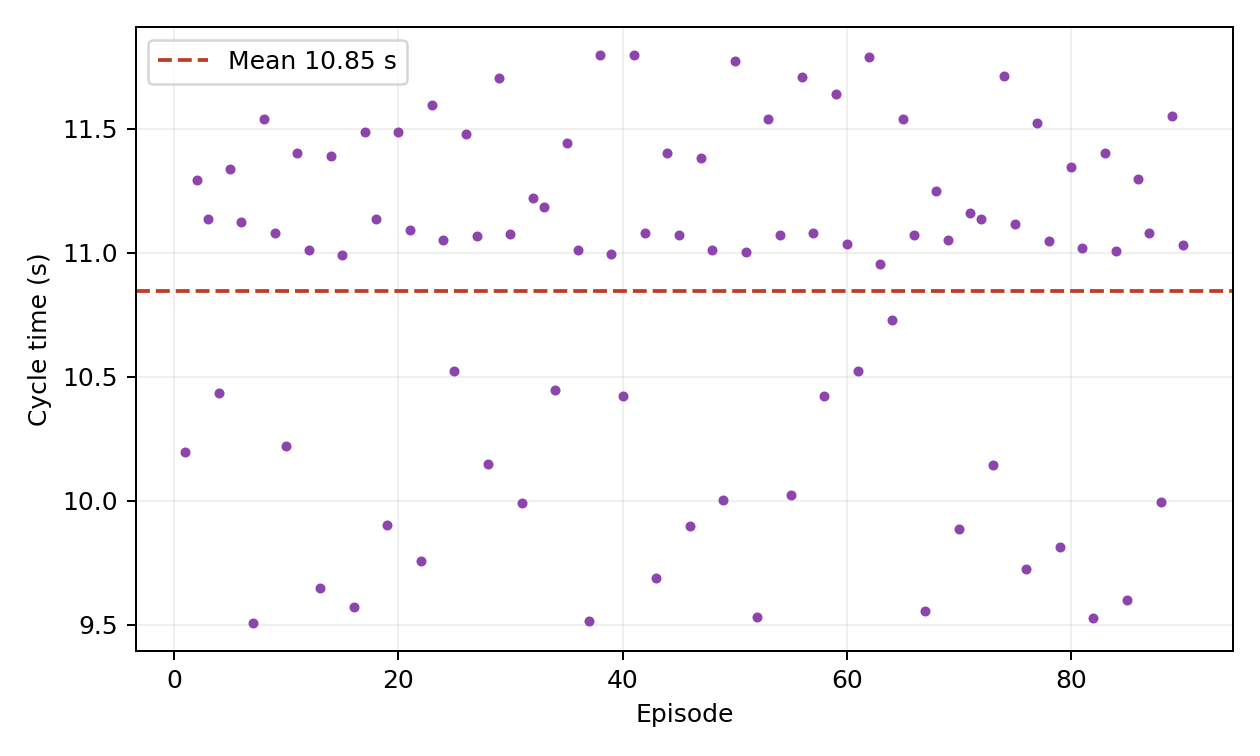
\includegraphics[width=\linewidth]{../outputs/gripper_main/cycle_time.png}\caption{逐轮周期}\end{subfigure}
\caption{主实验 \MainEpisodes\ 次随机初始化统计}\label{fig:charts}
\end{figure}
\enlargethispage{2\baselineskip}

\begin{figure}[H]\centering
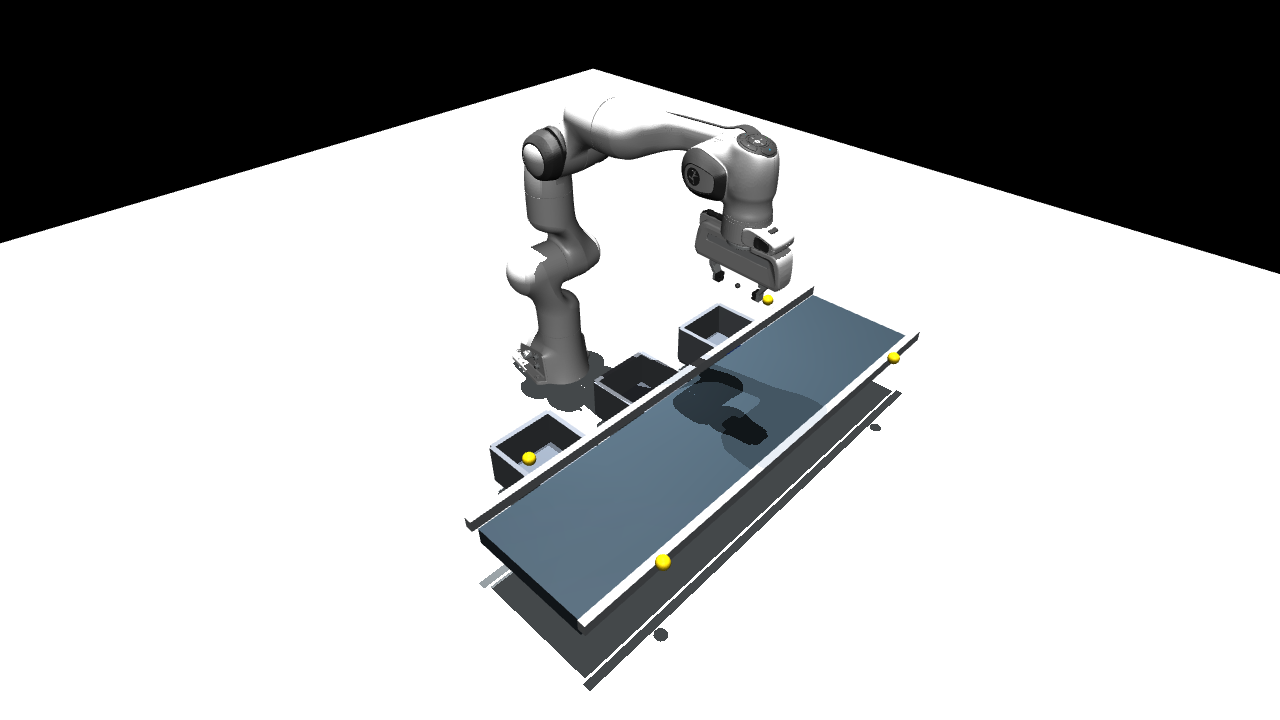
\includegraphics[width=0.64\linewidth]{../outputs/gripper_main/failure_case.png}
\caption{三棱柱投放失败回合的最终状态示例}\label{fig:failure}
\end{figure}

\subsection{转动与物理接触分析}
三类零件立方体、圆柱体和三棱柱的角速度峰值分别为 \DemoCubeOmega、\DemoCylinderOmega、\DemoPrismOmega\ rad/s；转运阶段，零件均保持在双指之间，代表典型抓取轨迹。对于随机姿态下的稳定性，我们再结合主实验统计：主实验中，各回合角速度峰值的平均值为 \MainMeanOmega\ rad/s，最大值为 \MainMaxOmega\ rad/s。相对手部旋转角峰值的平均值为 \MainMeanRelative$^\circ$，最大值为 \MainMaxRelative$^\circ$。在图\ref{fig:rotation}中给出两项指标的分布。

较大的角速度主要出现在三棱柱回合，包含成功与失败的情形，我们猜测这一过程中可能存在斜面接触引起的滑移或碰撞，但由于实验尚未记录峰值瞬间的接触点分布，其具体机制仍需进一步分析。

\begin{figure}[H]\centering
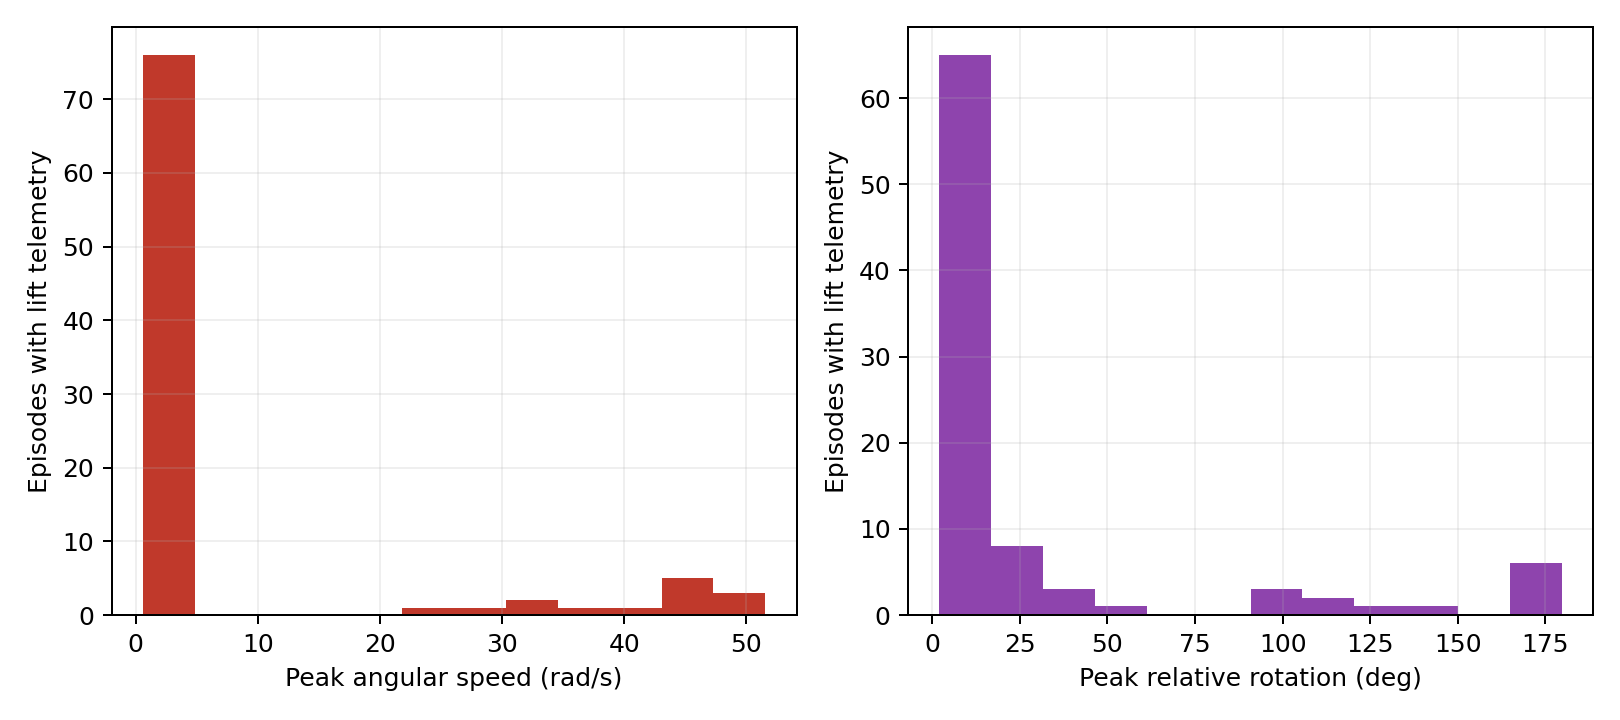
\includegraphics[width=0.82\linewidth]{../outputs/gripper_main/rotation.png}
\caption{主实验各回合抬升及转运阶段的物体角速度与相对手部姿态峰值}\label{fig:rotation}
\end{figure}

\subsection{真值位置、带速与光照对照}
表\ref{tab:ablation}比较了目标位置、带速和光照条件变化后的实验结果。其中，真值位置对照组正确入箱 \TruthCorrectCount/90，低于视觉主实验的 \MainCorrectCount/90；其中三棱柱正确入箱仅有 \TruthPrismCorrect/30。这组数据说明，目标接触位置与夹爪姿态也可能影响抓取结果。视觉质心与几何中心的微小差异可能改变三棱柱斜面的接触状态。当然，这个解释仍需通过控制抓取朝向与接触点的实验验证。

另一情形下，当带速为 $0.08$、$0.16$ m/s 时，系统分别正确入箱 \SpeedSlowCorrectCount/30 和 \SpeedFastCorrectCount/30；如果光照比例降至 $0.6$ ，正确入箱则变为 \LightDimCorrectCount/30。

对于时长这一因素，主实验的平均周期为 \MainCycleSec\ s，高于我们最初设立的 $8$ s 目标。结合整个控制流程分析，带物转运限速、到位稳定等待和机械臂返程等因素都可能影响周期。后续如想进一步缩短时间，可尝试优化轨迹、并行动作，再用独立实验量化收益。

\begin{table}[H]\centering\small
\caption{不同目标位置、带速与光照条件下的性能比较}\label{tab:ablation}
\begin{tabular}{lcccc}
\toprule 条件 & 回合 & 平面误差/mm & 正确入箱 & 平均周期/s\\\midrule
视觉主实验，$v=0.12$ & \MainEpisodes & \MainPositionMm & \MainCorrectCount/\MainEpisodes & \MainCycleSec\\
真值位置，$v=0.12$ & 90 & 0 & \TruthCorrectCount/90 & \TruthCycleSec\\
视觉，$v=0.08$ & 30 & \SpeedSlowPositionMm & \SpeedSlowCorrectCount/30 & \SpeedSlowCycleSec\\
视觉，$v=0.16$ & 30 & \SpeedFastPositionMm & \SpeedFastCorrectCount/30 & \SpeedFastCycleSec\\
视觉，光照0.6 & 30 & \LightDimPositionMm & \LightDimCorrectCount/30 & \LightDimCycleSec\\\bottomrule
\end{tabular}
\end{table}

\section{总结与展望}
我们设计并验证了间歇式输送线零件视觉识别与分类抓取系统。系统利用固定 RGB 相机与平面标定确定抓取目标，再由 Panda 双指夹爪在逆运动学和状态机控制下完成取放。在 $90$ 次随机初始化实验中，识别准确率为 \MainRecognitionPct\pct，平面定位平均误差为 \MainPositionMm\ mm；抬升成功率为 \MainGraspPct\pct，正确入箱率为 \MainSortPct\pct。这四项结果达到相应设计指标。只有平均周期为 \MainCycleSec\ s，仍高于 $8$ s 的目标值。

三棱柱的投放失败和部分回合的较大转动告诉我们，固定夹爪朝向对不规则零件的接触姿态适应性有限。后续如果想要提升本设计系统的性能，可以加入图像中的抓取朝向的估计，并加入接触力与滑移监测等功能。此外，还可研究连续轨迹规划和不停带预测抓取，提高复杂工况下的稳定性与作业效率。

\clearpage
\begin{thebibliography}{9}
\bibitem{mujoco_xml} Google DeepMind, \emph{MuJoCo XML Reference}, \url{https://mujoco.readthedocs.io/en/latest/XMLreference.html}。
\bibitem{menagerie} Google DeepMind, \emph{MuJoCo Menagerie}, \url{https://github.com/google-deepmind/mujoco_menagerie}。
\bibitem{panda} Google DeepMind, \emph{Franka Emika Panda MJCF}, \url{https://github.com/google-deepmind/mujoco_menagerie/blob/main/franka_emika_panda/panda.xml}。
\bibitem{opencv_h} OpenCV, \emph{Basic concepts of the homography explained with code}, \url{https://docs.opencv.org/4.5.1/d9/dab/tutorial_homography.html}。
\end{thebibliography}

\appendix
\section{项目组成员分工}


\begin{table}[H]\centering\small
\caption{项目组成员分工}\label{tab:member-info}
\begin{tabular}{clllllll}\toprule 序号 & 姓名 & 班级 & 学号 & 电话 & e-mail & 签字 & 独立承担内容\\\midrule
1 & 张令熙 & 机器人2301班 &  &  &  & &  \\
2 & 芮易成 & 机器人2301班 &  &  &  & &  \\
3 & 蒋中涛 & 机器人2301班 &  &  &  & &  \\
4 & 张梓峻 & 机器人2301班 &  &  &  & &  \\
5 & 杜彦宁 & 先进电子制造2301班 &  &  &  &  &  \\\bottomrule\end{tabular}
\end{table}
\end{document}
